\documentclass[12pt]{article}

\usepackage{mathrsfs}
\usepackage{epsfig}
\usepackage{graphicx}
\usepackage{color}
\usepackage{amsmath}
\usepackage{amsfonts}
\usepackage{amssymb}
\usepackage{amsthm}
\usepackage{amscd}
\usepackage{verbatim}
\usepackage{fullpage}
\usepackage{indentfirst}

%\setcounter{MaxMatrixCols}{20}
\theoremstyle{plain}
\newtheorem{theorem}{Theorem}[section]
\newtheorem{proposition}[theorem]{Proposition}
\newtheorem{lemma}[theorem]{Lemma}
\newtheorem{corollary}[theorem]{Corollary}
\newtheorem{conjecture}[theorem]{Conjecture}
\theoremstyle{definition}
\newtheorem{definition}[theorem]{Definition}
\newtheorem{notation}[theorem]{Notation}
\newtheorem{remark}[theorem]{Remark}
\newtheorem{example}[theorem]{Example}
\numberwithin{equation}{theorem}

\newcommand{\black}{\hfill{\ensuremath{\blacksquare}}}
\DeclareMathAlphabet{\mathpzc}{OT1}{pzc}{m}{it}

\graphicspath{ {./} }

\begin{document}
\begin{titlepage}
	\centering
	\vspace{4cm}
	{\scshape\Large DSE 210\par}
	\vspace{1.5cm}
	{\huge\bfseries Homework 4\par}
	\vspace{2cm}
	{\Large\itshape Kevin Kannappan\par}

% Bottom of the page
	{\large \today\par}
\end{titlepage}


\section{Generative models 3}
\subsection{Worksheet 8}
\begin{enumerate}
\item $4y - 3x \geq 12$ in $\mathbb{R}^{2}$. Hence, $y \geq \frac{3}{4}x + 3$. Drawn below:
\bigskip
\begin{center}
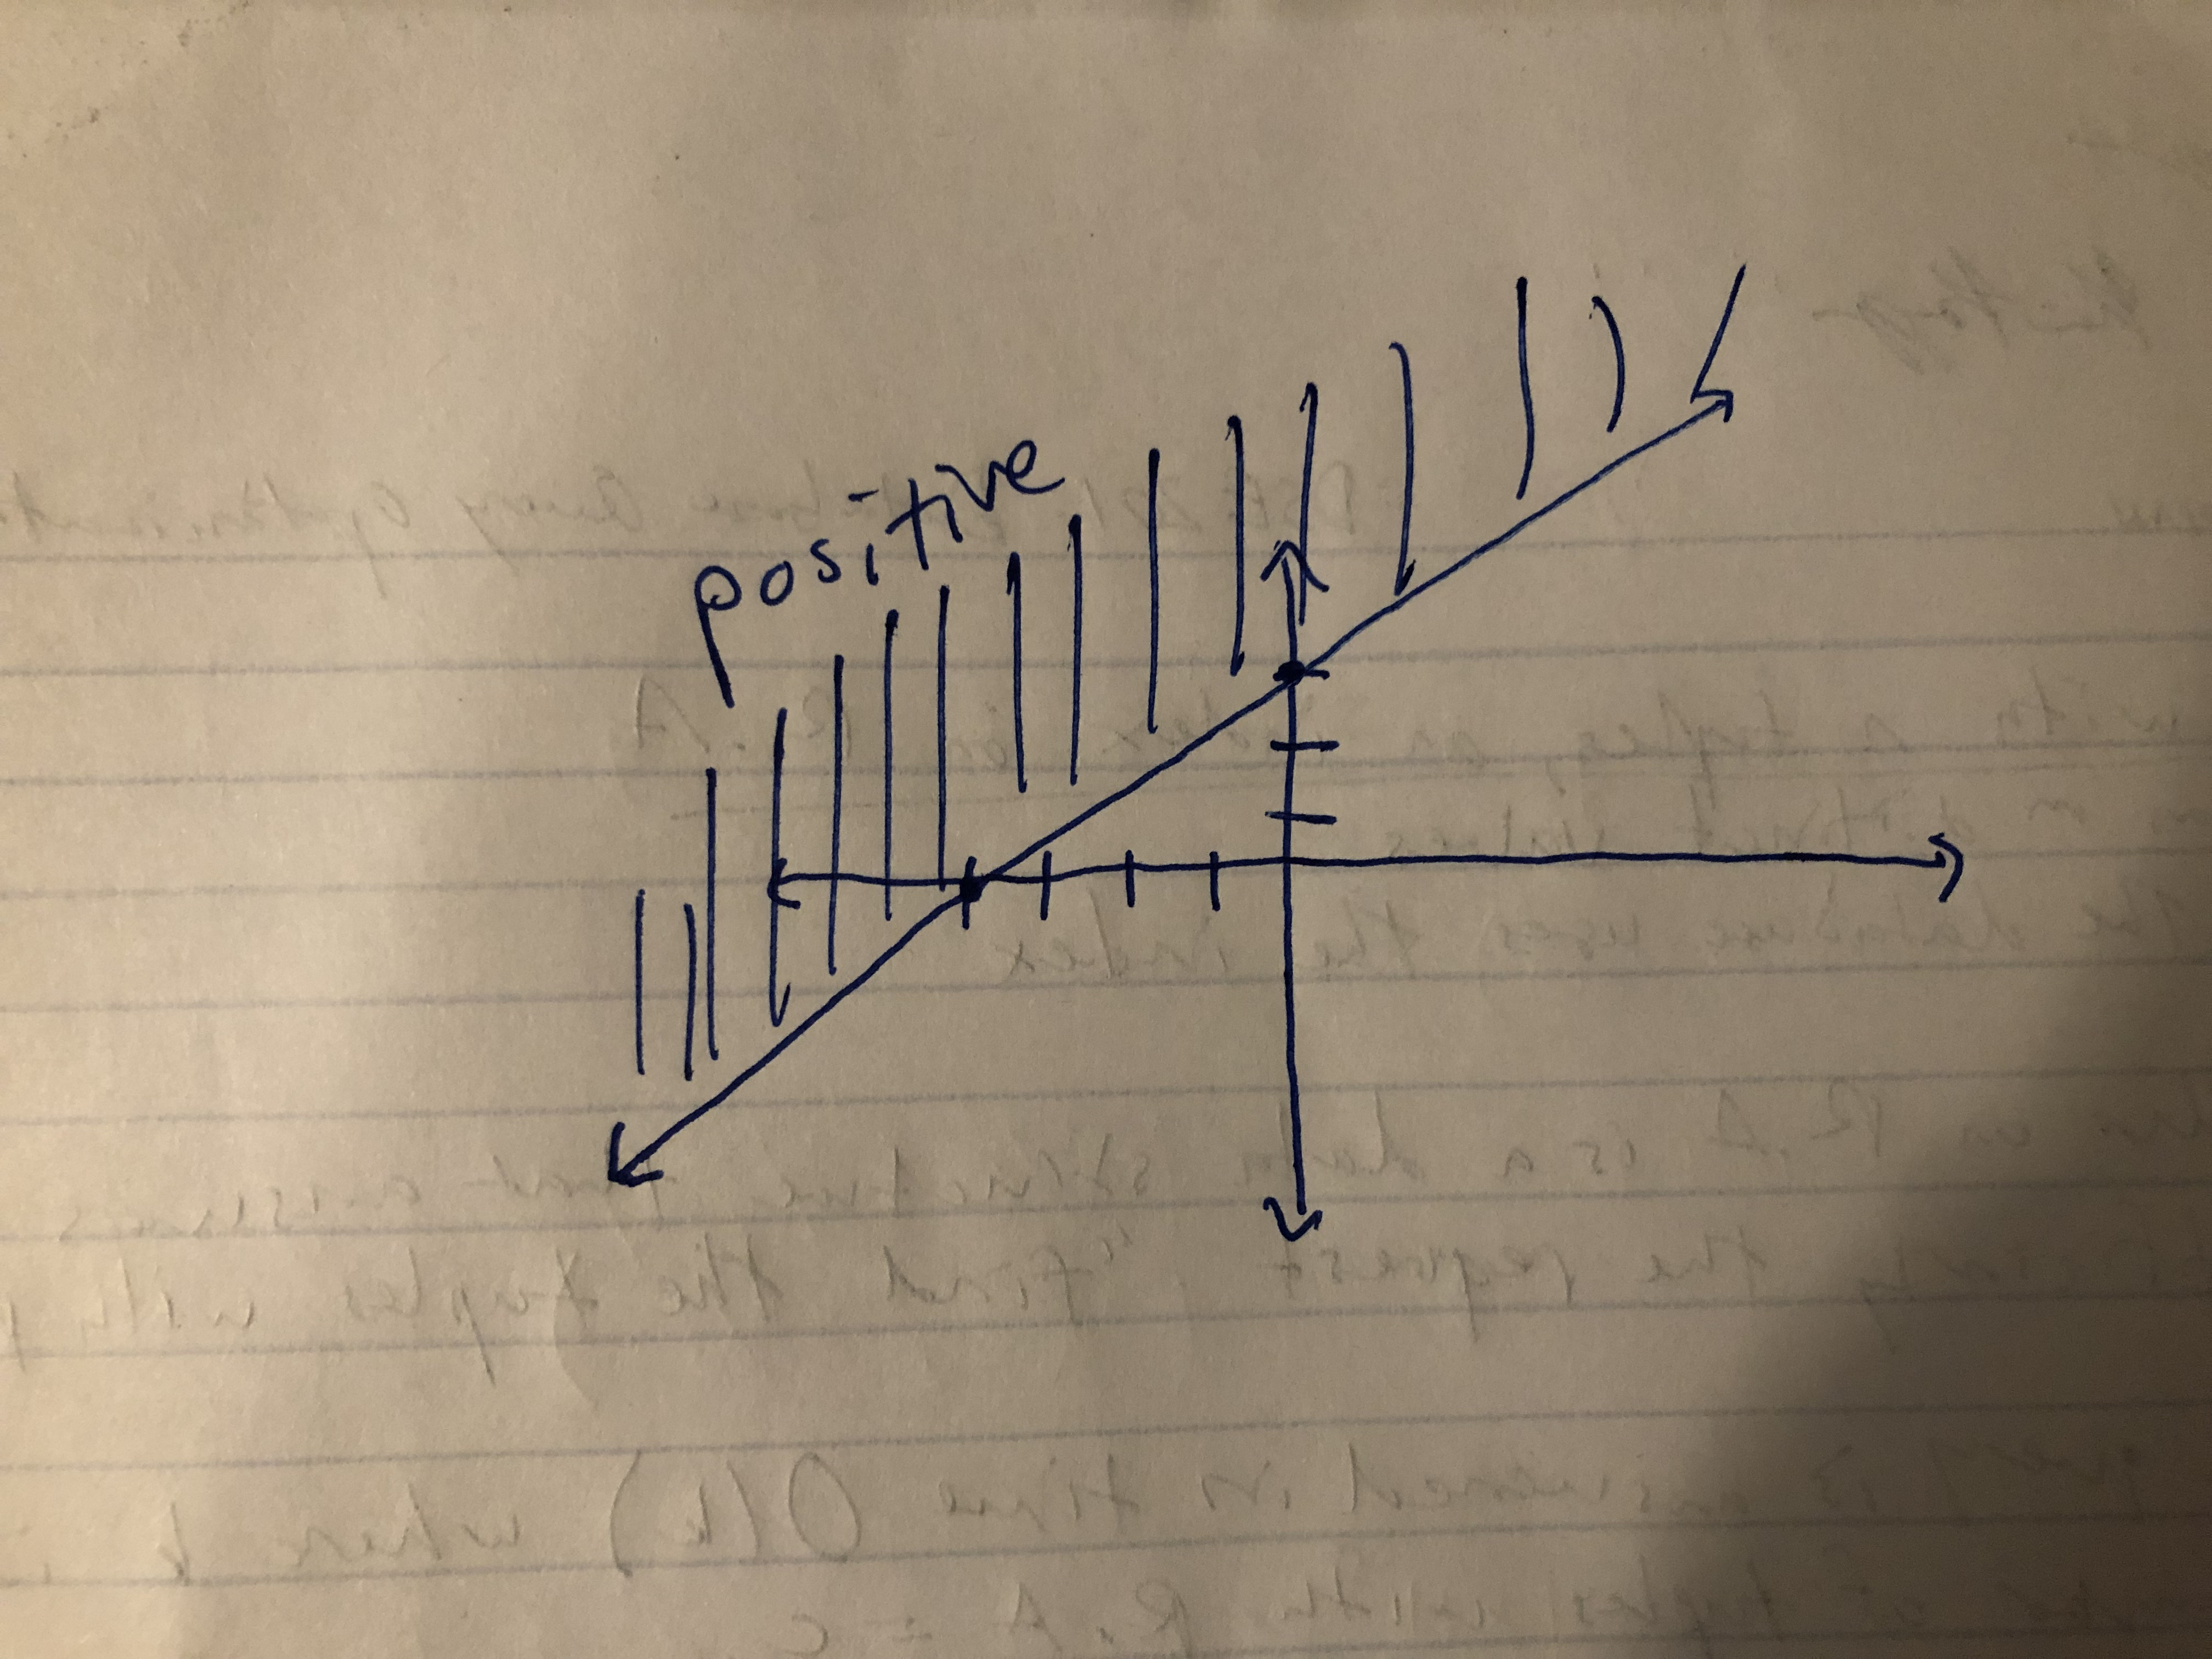
\includegraphics[width=12cm, height=9cm]{ws_8_q1}
\end{center}
\bigskip
\item $2d$. There are $d$ means and $d$ variances for a diagonal Gaussian in $\mathbb{R}^{d}$ and no covariances.
\item Please refer to Jupyter notebook for Problem 3.
\end{enumerate}
\bigskip

\section{PCA and SVD}
\subsection{Worksheet 10}
\begin{enumerate}
\addtocounter{enumi}{2}
\item
	\begin{enumerate}
	\item $U = d \times 2$. $U^{T} = 2 \times d$.  $UU^{T} = d \times d$.  $u_{1}u_{1}^{T} = d \times d$.
	\item Not entirely sure how to phrase the answer for this question, yet I will do my best to explain. In the first case, we have mapped unit vectors onto $x$. In the second case, we have taken those projections and mapped them in the directions of our unit vectors,  $u_{1}, u_{2}$. In the third case, we are effectively doing the same thing as we did in the first case, by transposing $U$ and mapping onto $x$ - may have formally different dimensions but I believe they are more or less similar. The last case we are taking our $d \times d$ unit vector matrix and mapping that to $x$, which I believe is similar to the second case - may have formally different dimensions.
	\end{enumerate}
\item Please refer to Jupyter notebook for Problem 4.

\end{enumerate}
\bigskip


\end{document}